\documentclass{article}


\usepackage{arxiv}

\usepackage[utf8]{inputenc} % allow utf-8 input
\usepackage[T1]{fontenc}    % use 8-bit T1 fonts
\usepackage{hyperref}       % hyperlinks
\usepackage{url}            % simple URL typesetting
\usepackage{booktabs}       % professional-quality tables
\usepackage{amsfonts}       % blackboard math symbols
\usepackage{amsmath}
\usepackage{nicefrac}       % compact symbols for 1/2, etc.
\usepackage{microtype}      % microtypography
\usepackage{lipsum}		% Can be removed after putting your text content
\usepackage{graphicx}
\usepackage{tikz}
\usepackage{multicol}
\usepackage{natbib}
\usepackage{doi}



\title{Boosting ARTM with PyTorch}

%\date{September 9, 1985}	% Here you can change the date presented in the paper title
%\date{} 					% Or removing it

\author{ \hspace{1mm} Ilya Diyakov \\
	Department of Mathematical Methods of Forecasting\\
	Moscow State University\\
	Moscow \\
	\texttt{s02210378@gse.cs.msu.ru} \\
	%% examples of more authors
	\And
	\hspace{1mm} Konstantin Vorontsov \\
	Department of Mathematical Methods of Forecasting\\
	Moscow State University\\
	Moscow \\
	\texttt{vokov@forecsys.ru} \\
	%% \AND
	%% Coauthor \\
	%% Affiliation \\
	%% Address \\
	%% \texttt{email} \\
	%% \And
	%% Coauthor \\
	%% Affiliation \\
	%% Address \\
	%% \texttt{email} \\
	%% \And
	%% Coauthor \\
	%% Affiliation \\
	%% Address \\
	%% \texttt{email} \\
}

% Uncomment to remove the date
%\date{}

% Uncomment to override  the `A preprint' in the header
%\renewcommand{\headeright}{Technical Report}
%\renewcommand{\undertitle}{Technical Report}
\renewcommand{\shorttitle}{Boosting ARTM with PyTorch}

%%% Add PDF metadata to help others organize their library
%%% Once the PDF is generated, you can check the metadata with
%%% $ pdfinfo template.pdf
\hypersetup{
pdftitle={A template for the arxiv style},
pdfsubject={q-bio.NC, q-bio.QM},
pdfauthor={David S.~Hippocampus, Elias D.~Striatum},
pdfkeywords={First keyword, Second keyword, More},
}

\begin{document}
\maketitle

\begin{abstract}
	Topic modelling is a fast and efficient technique for text analysis. Currently, the most popular approaches for topic modelling are BPTM (bayesian probabilistic topic models) and ARTM (additive regularization for topic modelling). Recently, a new emerging field, \emph{neural topic modelling}, became an increasingly popular research area. ARTM is a newer approach to this problem compared to LDA, and it has shown recent success in solving many applied problems in this area. The state-of-the-art model for ARTM is currently BigARTM, which uses the expectation-maximization algorithm. In this paper, we propose a different approach for solving the ARTM optimization problem, making use of the popular PyTorch Autograd framework for efficient implementation.
\end{abstract}


% keywords can be removed
\keywords{Clusterization \and Topic Modelling \and ARTM}


\section{\centering Introduction}
\label{sec:introduction}
Topic modeling is a relatively new approach to text analysis and clustering, which has shown success in many applications in these areas. Approaches emerging during the researches in NLP area also proved useful in a wide variety of problems from other domains like analysis of banking transaction data, image annotation or search for motifs in nucleotide and amino acid sequences. It makes topic modelling an efficient and universal approach for summarization, generalization, and extraction of specific features from unstructured data. \\

BPTMs, that generates the data from the pre-specified distributions, have been the most popular and successful representation of topic models. However, such approach has several significant drawbacks: \textbf{1)} Due to the use of specific pre-defined distributions in each problem, success in one problem cannot be easily generalized to the whole area or transferred to another area. \textbf{2)} The solution stability of BPTMs cannot be guaranteed. \textbf{3)} The scaling of trained model's inference or making use of parallel computing and GPUs is a challenging task. \textbf{4)} There is no modular realization of proposed models, so it is hard to add regularization to an already solved problem. \\

One of the main advantages of ARTM over BPTM is that its theoretical basis is easy to understand. ARTM successes in creating topic modelling algorithms which can be easily interpreted and scaled. There is also no need for a prior knowledge of the structure of data we are working with. These advantages make it a good alternative for Bayesian approach. Our research is aimed at improving speed and quality of the state-of-the-art model for ARTM, BigARTM. Our new model outperforms BigARTM in speed, maintaining the quality. For better understanding of our new approach, we first outline some theoretical background. \\


\section{\centering Theoretical Background}
\label{sec:theoretical-background}
Let us define the problem ARTM states and overview the solution of this problem proposed in BigARTM model. Then, we will propose a different approach for solving the same problem and compare these solutions.\\

\subsection{The classic problem of topic modelling}
Given the collection of documents $D$ with vocabulary $W$, described as a conditional distribution
\begin{equation}
    p(w|d) = \frac{n_{dw}}{n_{d}} \quad w \in W, d \in D,
\end{equation}
where $n_{dw}$ is the number of occurrences of the word $w$ in the document $d$, and $n_{d}$ is the total number of words in the document $d$. This distribution can be rewritten as
\begin{equation}
    p(w|d) = \sum_{t \in T}p(w|t)p(t|d) = \sum_{t \it T} \phi_{wt}\theta_{td} \quad w \in W, d \in D,
\end{equation}
where $T$ is the set of topics we want to extract. As can be seen from the equation, the number of topics can be varied and the content of each topic will change accordingly. The aim is to find conditional distributions $p(w|t)$ and $p(t|d)$ in the form of matrices $\Phi$ and $\Theta$ given the distribution $p(w|d)$. 

\subsection{ARTM Problem Statement}
The proposed problem is the problem of stochastic matrix factorization. For it to have a unique solution, it has to be regularized as follows:
\begin{equation}
    \sum_{d, w} n_{dw} \ln \sum_{t} \phi_{wt}\theta_{td} + R(\Phi, \Theta) \rightarrow \max_{\Phi, \Theta}
    \label{likelihood}
\end{equation}
Where $R(\Phi, \Theta$ --- additive regularization term. This is the classic problem of ARTM. BigARTM authors proposed a solution using expectation-maximization algorithm:
\begin{equation}
    \begin{cases}
        p_{tdw} \equiv p(t|d, w) = \underset{t \in T}{norm} \\
        \phi_{wt} = \underset{w \in W}{norm}\left(n_{wt} + \phi_{wt}\frac{\partial R}{\partial \phi_{wt}}\right), \quad n_{wt} = \underset{d \in D}{\sum} n_{dw}p_{tdw} \\
        \theta_{td} = \underset{t \in T}{norm}\left(n_{td} + \theta_{td}\frac{\partial R}{\partial \theta_{td}}\right), \quad n_{td} = \underset{w \in d}{\sum} n_{dw}p_{tdw} \\
    \end{cases}
    \label{em}
\end{equation}
Authors have proposed several technical optimizations for the algorithm, but the approach remained the same. Note, that on the maximization step, we have to find partial derivatives of regularization term. \\

Now, we can notice that the function we want to maximize \ref{likelihood}  can be easily optimized directly with any of the autograd frameworks. So our first new approach for solving this problem is to use PyTorch for automatic differentiation. Among other advantages of this approach (see \ref{sec:experiments}), it allows using custom user's regularization functions.

\section{\centering Implementation Details}
\label{sec:implementation}
The program provides compatibility with scikit-learn functions and provides the same interfaces for user. We tried to make our implementation easy-to-use for beginners and provide a clear and flexible framework for advanced users.\\

\begin{table}[htbp]
\centering
    \begin{tabular}{|c|c|c|}
        \hline
         & Proposed model & BigARTM \\
        \hline
        Parallel calculation on cpu     & No                & Yes \\
        \hline
        GPU enabled                     & Yes               & No \\
        \hline
        Input types                     & torch.Tensor,     & Vowpal Wabbit, \\
                                        & pandas.DataFrame  & UCI bow \\
        \hline
    \end{tabular}
\caption{Brief comparison of BigARTM and proposed model}
\label{tab:model-comparison}
\end{table}

It operates with more common torch \texttt{Tensor} and pandas \texttt{DataFrame} types, unlike BigARTM, which uses \texttt{Vowpal Wabbit} or \texttt{UCI bow} formats for input data. The main goal of the program is to provide functionality for future research in the field and draw attention of other researchers who needs a fast and reliable software for their work.\\

\begin{figure}[h]
\centering
    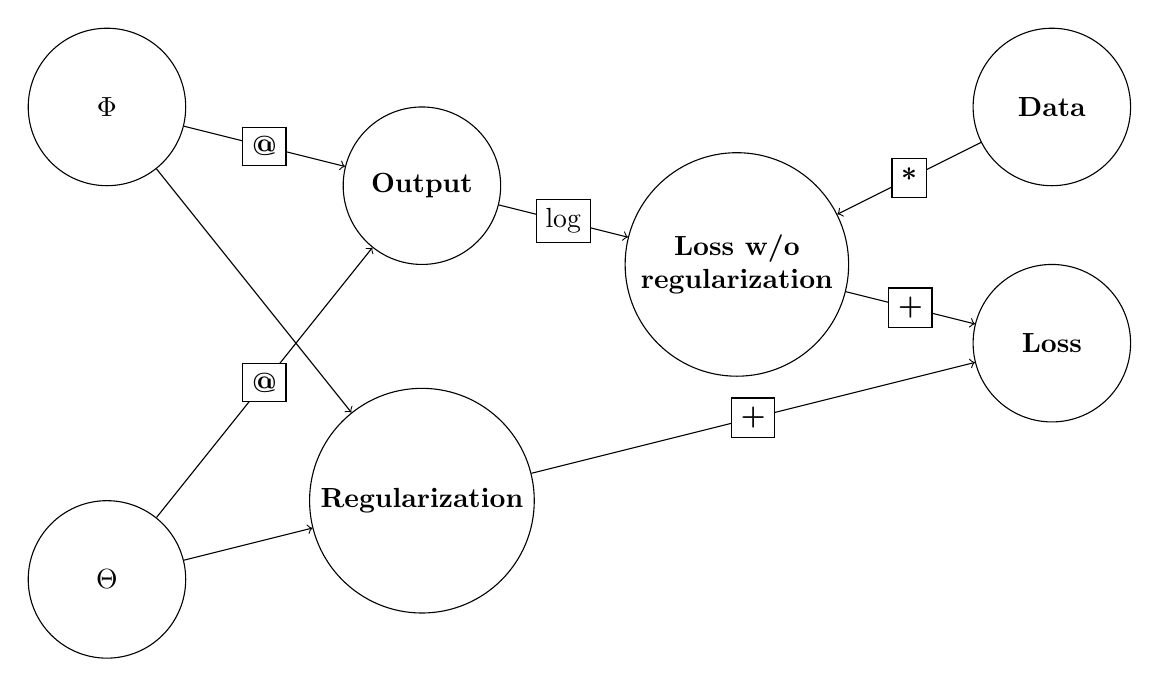
\begin{tikzpicture}[every node/.style={font=\bfseries}]
        \node[draw, circle, minimum size=2cm] (phi) at (0,0) {$\Phi$};
        \node[draw, circle, minimum size=2cm] (theta) at (0,-6) {$\Theta$};

        \node[draw, circle, minimum size=2cm] (output) at (4,-1) {Output};
        \node[draw, circle, minimum size=2cm] (reg) at (4,-5) {Regularization};

        \node[draw, circle, minimum size=1cm, align=center] (loss1) at (8,-2) {Loss w/o \\ regularization};

        \node[draw, circle, minimum size=2cm] (data) at (12,0) {Data};
        \node[draw, circle, minimum size=2cm] (loss2) at (12,-3) {Loss};

        \draw[->] (phi) -- (output) node[draw, rectangle, midway, fill=white] {@};
        \draw[->] (theta) -- (output) node[draw, rectangle, midway, fill=white] {@};
        \draw[->] (phi) -- (reg);
        \draw[->] (theta) -- (reg);

        \draw[->] (output) -- (loss1) node[draw, rectangle, midway, fill=white] {$\log$};

        \draw[->] (loss1) -- (loss2) node[draw, rectangle, midway, fill=white] {+};
        \draw[->] (reg) -- (loss2) node[draw, rectangle, midway, fill=white] {+};
        \draw[->] (data) -- (loss1) node[draw, rectangle, midway, fill=white] {*};
    \end{tikzpicture}
    \caption{Calculation graph}
    \label{fig:calc-graph}
\end{figure}
Our implementation of the proposed algorithm is lighter and easier to maintain, because most of the optimization falls on the PyTorch module. Also, with the support of PyTorch, we can utilize GPU for training. This makes inference much faster compared to BigARTM \ref{sec:experiments}.

\section{\centering Experiments}
\label{sec:experiments}
\subsection{Data}
We evaluate the proposed model on the 20newsgroups dataset, which contains a collection of approximately 20,000 newsgroup documents, partitioned nearly evenly across 20 different newsgroups. We extracted approximately 70,000 unique words as vocabulary in bag-of-words format.

\subsection{Quantitative Results}
We report our quantitative results in Table \ref{tab:quantitative-results}, training both models on 20 steps. Both models were compared without regularization (PLSA). To measure topic similarity, we used the Hungarian algorithm to find similar topics using cosine metric between top-3 words as distance between topics. Then we calculated the mean distance across all distances between the most similar topics. All metrics were aggregated over 100 runs. \\

\begin{table}[htbp]
\centering
    \begin{tabular}{|c|c|c|c|c|}
        \hline
        Metric & Ours, 10 topics & BigARTM, 10 topics & Ours, 120 topics & BigARTM, 120 topics \\
        \hline
        Perplexity@10step   & 3750 & 2600 & 2780 & 1170 \\
        \hline
        Perplexity@20step   & 2800 & 2520 & 1310 & 1120 \\
        \hline
        Perplexity@30step   & 2670 & 2500 & 1190 & 1110 \\
        \hline
        Training time CPU (30 steps, sec)  & 400 & 30 & 1400 & 130 \\
        \hline
        Training time GPU (30 steps, sec) & 40 & --- & 40 & --- \\
        \hline
        Topic similarity    & \multicolumn{2}{|c|}{0.65} & \multicolumn{2}{|c|}{0.4} \\
        \hline
    \end{tabular}
\caption{Quantitative results training BigARTM and proposed models}
\label{tab:quantitative-results}
\end{table}

Overall, our implementation shows very similar results with BigARTM, but successes in speeding up the inference with GPU. For both models, only 20 steps are sufficient to generate interpretable topics from the given data. Note that both models are producing many similar topics, which shows that the algorithm's principle remains the same. \\

The results show that our model's training time cannot compete with efficient CPU implementation of BigARTM, but on GPU it gains better results. Training time on GPU does not depend on number of topics because of efficient parallelization. This demonstrates the potential of the proposed model in large datasets.

\subsection{Qualitative Results}
Here, we analyze our results in terms of top k words, representing the topic, focusing on models with 10 topics. These particular examples demonstrate the same logic of clustering in both models.\\

\begin{multicols}{2}
\section*{BigARTM, top-5 topic words}
topic 1: max, q, r, g, p\\
topic 2: one, would, say, people, write\\
topic 3: game, team, line, subject, organization\\
topic 4: would, people, write, gun, article\\
topic 5: god, hell, atheist, line, subject\\
topic 6: x, file, use, window, program\\
topic 7: say, armenian, people, one, go\\
topic 8: line, subject, get, organization, car\\
topic 9: space, organization, subject, line, db\\
topic 10: line, subject, organization, use, university\\

\columnbreak

\section*{Ours, top-5 topic words}
topic 1: max, q, r, g, p\\
topic 2: line, one, get, subject, use\\
topic 3: god, would, say, one, people\\
topic 4: line, subject, organization, university, article\\
topic 5: game, team, line, drive, subject\\
topic 6: say, armenian, one, go, people\\
topic 7: x, file, line, use, subject\\
topic 8: use, line, subject, organization, window\\
topic 9: would, people, write, get, article\\
topic 10: use, key, system, data, space\\
\end{multicols}

\section{\centering Conclusion}
The proposed model seems to be a promising direction of development, offering accessibility and lightness to the user, the ability to flexibly configure system components and integrate custom regularizers. One of the most important advantages of the developed program is its efficiency. Also, the proposed algorithm can become the first step of ARTM's integration with deep neural networks. This can solve several crucial problems of modern neural networks. Among them, we can highlight the selection of the learning rate (ARTM does not need this parameter, \ref{sec:theoretical-background}) as well as the interpretability of the inner layers as a set of <<topics>>, which model extracts from data.

\begin{thebibliography}{20}

\bibitem{blei2003latent}
David~M Blei, Andrew~Y Ng, and Michael~I Jordan.
\newblock Latent dirichlet allocation.
\newblock {\em Journal of machine Learning research}, 3(Jan):993--1022, 2003.

\bibitem{yin2018neural}
Jiaqi Yin and Xin Liu.
\newblock Neural topic modeling with graph attention.
\newblock {\em arXiv preprint arXiv:1809.04348}, 2018.

\bibitem{zhao2018topic}
Haozheng Zhao, Zhou Yu, and Chong Wang.
\newblock Topic modeling with graph convolutional neural networks.
\newblock In {\em Proceedings of the 2018 Conference on Empirical Methods in Natural Language Processing}, pages 4231--4238, 2018.

\bibitem{vorontsov2015additive}
Konstantin~V Vorontsov.
\newblock Additive regularization of topic models.
\newblock {\em Machine Learning}, 101(1-3):449--470, 2015.

\bibitem{vorontsov2013probabilistic}
Konstantin~V Vorontsov and Alexander Potapenko.
\newblock Probabilistic topic models for text collection analysis.
\newblock In {\em International Conference on Analysis of Images, Social Networks and Texts}, pages 32--56. Springer, 2013.

\bibitem{vorontsov2014bigartm}
Konstantin~V Vorontsov, Alexey~A Potapenko, and Dmitry~A Plavin.
\newblock Bigartm: Open source library for regularized topic modeling.
\newblock In {\em Analysis of Images, Social Networks and Texts}, pages 145--152. Springer, 2014.

\bibitem{miao2016neural}
Yishu Miao, Lei Yu, and Phil Blunsom.
\newblock Neural variational inference for text modeling.
\newblock In {\em Proceedings of the 33rd International Conference on Machine Learning}, pages 1212--1221, 2016.

\bibitem{kingma2013auto}
Diederik~P Kingma and Max Welling.
\newblock Auto-encoding variational bayes.
\newblock {\em arXiv preprint arXiv:1312.6114}, 2013.

\bibitem{rezende2014stochastic}
Danilo~Jimenez Rezende, Shakir Mohamed, and Daan Wierstra.
\newblock Stochastic backpropagation and approximate inference in deep generative models.
\newblock In {\em Proceedings of The 31st International Conference on Machine Learning}, pages 1278--1286, 2014.

\bibitem{paszke2019pytorch}
Adam Paszke, Sam Gross, Francisco Massa, Adam Lerer, James Bradbury, Gregory Chanan, Trevor Killea, Zeming Lin, Nathaniel
  Gruman, et~al.
\newblock Pytorch: An imperative style, high-performance deep learning library.
\newblock In {\em Advances in neural information processing systems}, pages 8026--8037, 2019.

\bibitem{hoffman2013stochastic}
Matthew~D Hoffman, David~M Blei, and Francis Bach.
\newblock Stochastic variational inference.
\newblock {\em Journal of machine learning research}, 14(1):1303--1347, 2013.

\bibitem{roberts2018hierarchical}
Andrew Roberts, Adam  Gorman, and Yael  Sharir.
\newblock Hierarchical Neural Topic Models.
\newblock In {\em Proceedings of the 2018 Conference on Empirical Methods in Natural Language Processing},  2018.

\bibitem{li2017variational}
Xiao Li and Chris Callison-Burch.
\newblock Variational autoencoding for topic modeling.
\newblock In {\em Proceedings of the 55th Annual Meeting of the Association for Computational Linguistics}, pages 1370--1380, 2017.


\bibitem{xiao2019improving}
Lingwei Xiao, Yanping Zhang, and Liang Zhao.
\newblock Improving neural topic models with latent variable integration.
\newblock {\em Knowledge-Based Systems}, 186:104807, 2019.

\bibitem{chen2017variational}
Wray Chen, Siqi Liu, and Zhiyuan Liu.
\newblock Variational Neural Topic Model for Text Generation.
\newblock {\em International Journal of Semantic Computing}, 11(02):279--299, 2017.


\bibitem{gupta2019topic}
Ruchi Gupta and Prateek Bhatnagar.
\newblock Topic Modeling with Neural Networks.
\newblock In {\em Emerging Research in Data Engineering and Machine Learning}, pages 151--162. Springer, 2019.


\bibitem{battenberg2015reparameterization}
Eric Battenberg, Adam Lerer, and Daniel  Kahn.
\newblock The reparameterization trick for variational bayesian inference.
\newblock  {\em Neural Computation}, 2015.


\bibitem{johansson2020bayesian}
Fredrik Johansson, Martin Ljungkrantz, and Christopher Petersson.
\newblock Bayesian topic models: an approach for qualitative data analysis.
\newblock {\em Quality & Quantity}, 54(1): 291-313, 2020.

\bibitem{sharma2020neural}
Ashish Sharma, and Anupam Singh.
\newblock Neural Topic Modeling with BERT Embeddings.
\newblock In {\em Artificial Intelligence and Machine Learning: Second International Conference, AIML 2020}, pages 246--255. Springer, 2020.

\bibitem{yuan2020modeling}
Yuan, H. & Huang, X.
\newblock Modeling User Interests with Personalized Neural Topic Models.
\newblock In {\em International Conference on Smart Data and Intelligent Systems}, pages 118-124, 2020.

\end{thebibliography}


\end{document}
